\documentclass[pdftex,12pt,a4paper]{report}

\usepackage[dvipsnames]{xcolor}
\usepackage[pdftex]{graphicx}
\usepackage{float}
\usepackage{fancyvrb}
\fvset{xleftmargin=2em}

\usepackage{pgfplots}
\pgfplotsset{width=10cm,compat=1.9}
\usepackage{tikzscale}
\usepackage{pgfplotstable}
\usepackage{booktabs}
\usepackage[font=small,labelfont=bf,tableposition=top]{caption}

\usepackage[utf8]{inputenc}
\usepackage[portuges]{babel}
\usepackage[T1]{fontenc}
\usepackage{times}
%\usepackage{lmodern}
\usepackage[obeyspaces,spaces]{url}
\usepackage[left=20mm,right=20mm,top=25mm,bottom=25mm]{geometry}
\usepackage{titlesec}
\usepackage{mathtools}
\usepackage{amsfonts}

%identa 1º paragrafo de capitulos e secções
\usepackage{indentfirst}
\usepackage{url}
%\usepackage{alltt}
\usepackage[]{hyperref}
\usepackage{xspace}
\usepackage[final]{pdfpages}

\hypersetup{
%pdftitle={Trabalho 1 - Gestão de Projeto},
%pdfauthor={Bruno Pereira},
%pdfsubject={Investigação Operacional},
%pdfkeywords={keyword1, keyword2}},
bookmarksnumbered=true,     
bookmarksopen=true,         
bookmarksopenlevel=1,       
colorlinks=true,            
pdfstartview=Fit,           
pdfpagemode=UseOutlines, % this is the option you were lookin for
pdfpagelayout=TwoPageRight
		}

\usepackage{minted}
\usemintedstyle{borland}
\setminted{frame=lines,
framesep=2mm,
baselinestretch=1.2,
fontsize=\footnotesize,
linenos, 
breaklines,
breakautoindent=false,
autogobble
}
\usepackage{caption}

\begin{document}

\begin{titlepage}
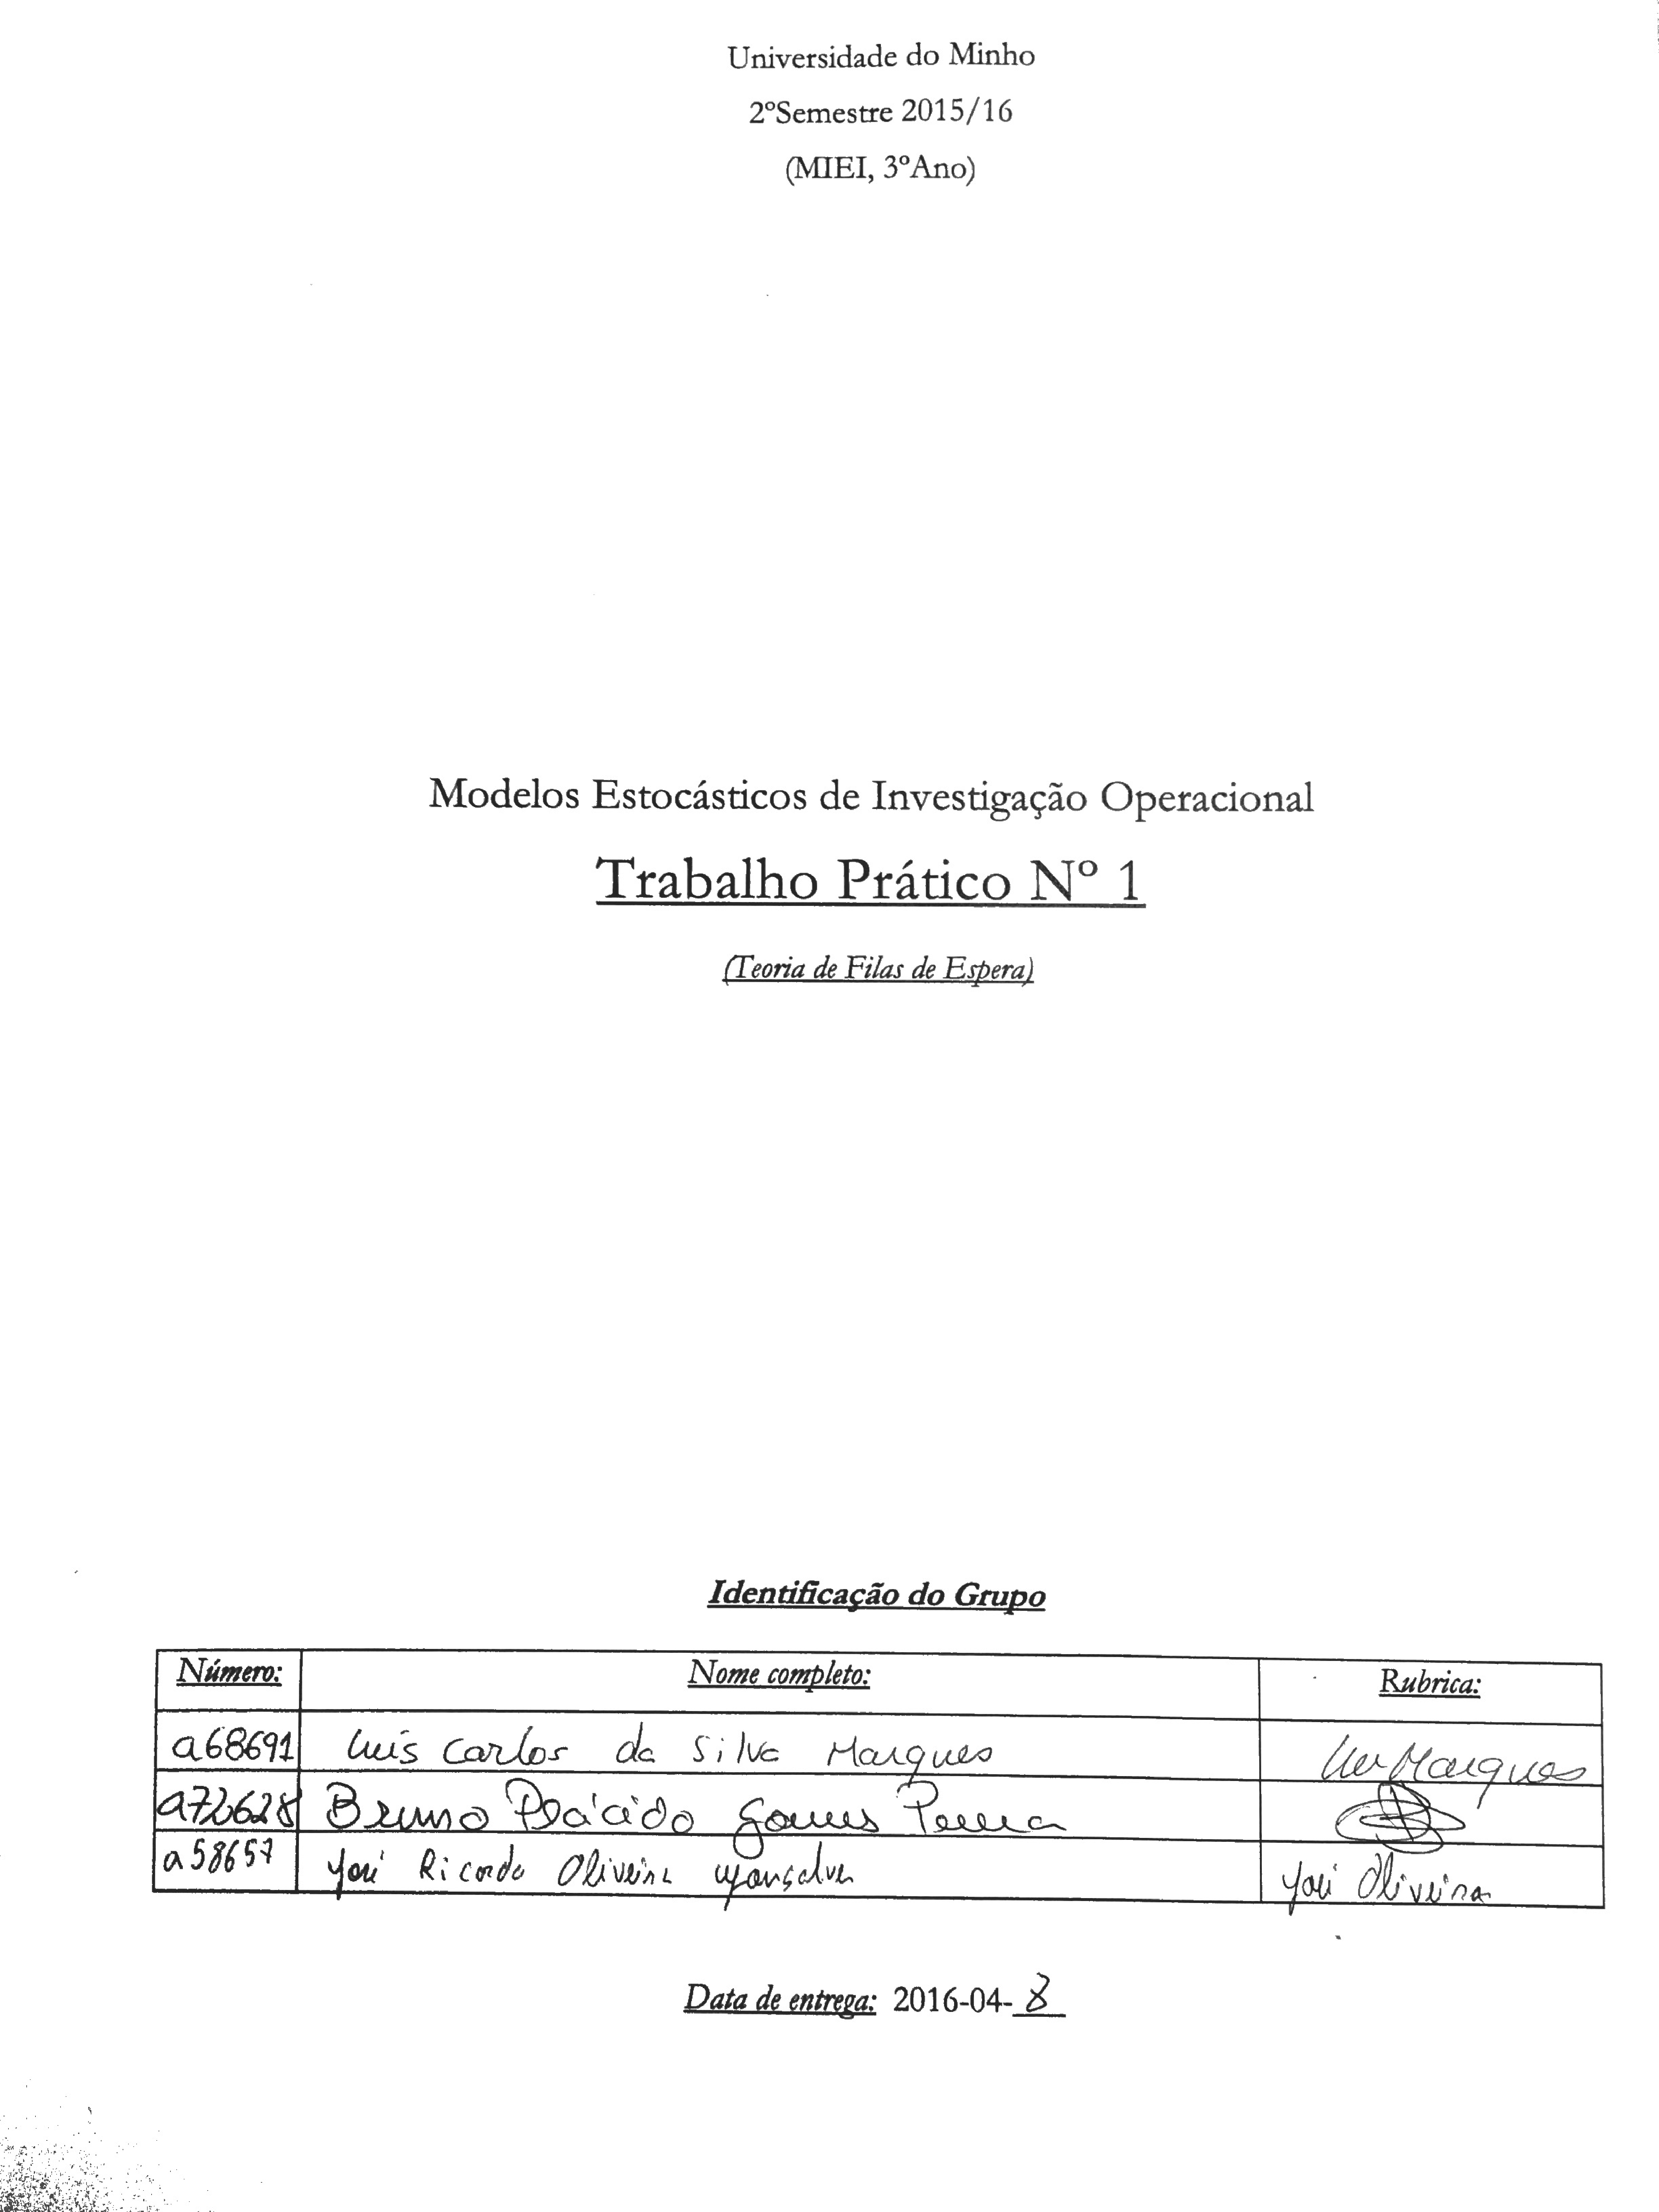
\includepdf[pages={1}]{./report/front.pdf}


\end{titlepage}






\begin{abstract}





\end{abstract}

\tableofcontents
\chapter*{Introdução}
\label{cap:intro}



\chapter{Parte 1}
\label{cap:p1}




\section{Dimensionamento do serviço de clientes}

\subsection{Análise do problema}
\subsubsection{Dados}
\subsubsection{Cálculos}





\newpage
\subsection{Testes e Resultados}


\section{Pressupostos considerados}






\chapter{Parte 2}
\label{cap:p2}

\section{Resumo de artigo}

\subsection{Teoria de filas de espera aplicadas a simulações de performance de
	\emph{Cloudcomputing}}\footnote{\url{http://www.dbjournal.ro/archive/20/20_7.pdf}}



Este artigo introduz os conceitos de teoria de filas de espera e processos
estocásticos aplicáveis à modelação de performance computacional, comparando no
final os resultados obtidos através da solução matemática com os resultados
obtidos através da simulação por software de um modelo de filas de espera.
   
Inicialmente, é descrito de uma formal geral o processo de \emph{Poisson},
correspondente ao registo e contagem dos intervalos de tempo entre a ocorrência
de eventos independentes. Considerando um processo em que tais eventos ocorrem
de forma aleatória, a distribuição exponencial é a função necessária para
descrever tal processo. O autor defende a importância da distribuição
exponencial na simulação de performance computacional, usando como exemplo
a modelação da chegada de pedidos a um servidor, no qual se pode assumir que os
pedidos são gerados de forma aleatória e independente.

Para a futura análise da aplicabilidade de uma simulação computacional, o autor
considera um modelo de fila de espera \emph{M/G/1}, ou fila de espera com distribuição
genérica. Este modelo usa uma distribuição exponencial para descrever taxa de
chegada de pedidos ao sistema, com um tempo de atendimento aleatório.
A utilização da teoria das filas de espera permite determinar o tempo médio que
um pedido espera na fila antes de ser servido, que corresponde à total dos
tempos de atendimento para cada pedido à frente do pedido considerado, somado
com o tempo de atendimento restante do pedido que é servido no momento da
chegada do pedido considerado à fila. O autor apresenta também os processos
matemáticos para a medição de performance no modelo \emph{M/G/1}, usando uma taxa de
chegada lambda e um tempo de atendimento X para determinar a utilização do
sistema. 

Seguidamente, o autor descreve a criação do algoritmo para modelar os sistema
\emph{M/G/1}, referindo o uso do método da transformada inversa para a geração de
tempos de intervalo entre chegadas e tempos de atendimento aleatórios.
Consequentemente o autor procede à comparação entre a solução matemática
e a simulação informática deste problema de filas de espera, com o objetivo de
testar a aplicabilidade da último. A simulação é testada com quatro
distribuições de tempo de chegada diferentes, e confirma a precisão do modelo de
simulação ao verificar que os valore obtidos estão de acordo com os resultados
das soluções matemáticas para as quatro distribuições testadas.

O autor conclui por fim, que o a simulação computacional é uma ferramenta
importante para a análise de modelos de filas de espera, principalmente em casos
de maior complexidade em que a aproximação matemática pode ser não prática.





\chapter*{Conclusão}
\label{cap:concl}




\appendix

\chapter{Código do Programa}




\begin{verbatim}

public class Aula()

  {

    int n, m;

    int max(int a, int b)

      {

       ......

       return(max);

      }

  }

\end{verbatim}



\begin{verbatim}

llll sanjdb c kjnjcnjnjj mmmmmmmmmmmmm hhhhhhhhhhhhhhhhhhhhhhhh
jjjjjjjjjjjjjjjjjjjjjjjjjjjj kkkkkkkkkkkkkkkkkk

      aqui deve aparecer o código do programa,

      tal como está formato no ficheiro-fonte "darius.java"

      caso indesejável $\varepsilon$

\end{verbatim}



\begin{minted}{c}

#include <stdio.h>
#define N 10
/* Block
 * comment */

 int main()
 {
     int i;
	 
	   // Line comment.
		 puts("Hello world!");
			     
		 for (i = 0; i < N; i++)
		 {
		 puts("LaTeX is also great for programmers!");
		 }
										 
	   return 0;
				
}
\end{minted}


E ainda possível importar diretamente o ficheiro:


%\begin{longlisting}
%	\inputminted{c}{Exercicio2/exe2_1.l}
%	\caption{Ficheiro fonte do exercício 2.1}
%	\label{listing:3}
%\end{longlisting}





\bibliographystyle{alpha}

\bibliography{./report/bibs/pl}

\end {document}


